\documentclass[12pt,letterpaper]{article}
\usepackage{fullpage}
\usepackage[top=2cm, bottom=4.5cm, left=2.5cm, right=2.5cm]{geometry}
\usepackage{amsmath,amsthm,amsfonts,amssymb,amscd}
\usepackage{lastpage}
\usepackage{enumerate}
\usepackage{fancyhdr}
\usepackage{mathrsfs}
\usepackage{xcolor}
\usepackage{graphicx}
\usepackage{listings}
\usepackage{hyperref}
\usepackage[T1]{fontenc}
\usepackage{textcomp}

\hypersetup{
  colorlinks=true,
  linkcolor=blue,
  linkbordercolor={0 0 1}
}

\definecolor{limitblue}{RGB}{32, 76, 113}
\definecolor{ruddybrown}{rgb}{0.73, 0.4, 0.16}
\colorlet{punct}{red!60!black} 
\definecolor{background}{HTML}{EEEEEE}
\definecolor{delim}{RGB}{20,105,176}
\definecolor{ogreen}{rgb}{0.0, 0.5, 0.0}
\colorlet{numb}{magenta!60!black}
 
\renewcommand\lstlistingname{Code}
\renewcommand\lstlistlistingname{Codes}
\def\lstlistingautorefname{Alg.}

\lstdefinestyle{Python}{
  language        = Python,
  frame           = lines, 
  basicstyle      = \footnotesize,
  keywordstyle    = \color{blue},
  stringstyle     = \color{green},
  commentstyle    = \color{red}\ttfamily
}
\lstdefinestyle{R}{
  language        = R,
  frame           = lines,
  captionpos      = b,
  abovecaptionskip= 10pt, 
  emphstyle       = \textbf,
  framextopmargin = 4pt,
  framexbottommargin = 4pt,
  basicstyle      = \ttfamily\footnotesize,
  keywordstyle    = \color{limitblue},
  stringstyle     = \color{ruddybrown},
  showstringspaces= false,
  commentstyle    = \color{red}\ttfamily,
  tabsize         = 2,
  literate=
    *{0}{{{\color{numb}0}}}{1}
      {1}{{{\color{numb}1}}}{1}
      {2}{{{\color{numb}2}}}{1}
      {3}{{{\color{numb}3}}}{1}
      {4}{{{\color{numb}4}}}{1}
      {5}{{{\color{numb}5}}}{1}
      {6}{{{\color{numb}6}}}{1}
      {7}{{{\color{numb}7}}}{1}
      {8}{{{\color{numb}8}}}{1}
      {9}{{{\color{numb}9}}}{1}
      {:}{{{\color{punct}{:}}}}{1}
      {,}{{{\color{punct}{,}}}}{1}
      {\{}{{{\color{delim}{\{}}}}{1}
      {\}}{{{\color{delim}{\}}}}}{1}
      {[}{{{\color{delim}{[}}}}{1}
      {]}{{{\color{delim}{]}}}}{1}
}

\setlength{\parindent}{0.0in}
\setlength{\parskip}{0.05in}

% Edit these as appropriate
\newcommand\course{Statistics I}
\newcommand\hwnumber{5.1}                  % <-- homework number
\newcommand\NetIDa{Atreya Choudhury}           % <-- NetID of person #1
\newcommand\NetIDb{bmat2005}           % <-- NetID of person #2 (Comment this line out for problem sets)

\pagestyle{fancyplain}
\headheight 35pt
\lhead{\NetIDa}
\lhead{\NetIDa\\\NetIDb}                 % <-- Comment this line out for problem sets (make sure you are person #1)
\chead{\textbf{\Large Assignment \hwnumber}}
\rhead{\course \\ \today}
\lfoot{}
\cfoot{}
\rfoot{\small\thepage}
\headsep 2em

\begin{document}
\textit{1}
\textit{Find the hypergeometric probability mass function (pmf) for m=100, n=200, k=5. [Here m is the number of white balls, n is the number of black balls and k is the number of balls drawn, that is sample size. The random variable is the number of white balls in the sample.]}

\textbf{Answer:}\\
The hypergeometric probability mass function for the given setup is given by:
$$p_H(x) = \frac{{100 \choose x}{200 \choose {5-x}}}{{300 \choose 5}}$$
\vspace{2em}

\textit{Find the binomial probability distribution for n=5 and p=1/3.}\\
\textbf{Answer:}\\
The binomial probability mass function for the given setup is given by:
$$p_B(x) = {5 \choose x}\biggl(\frac{1}{3}\biggr)^x\biggl(\frac{2}{3}\biggr)^{5-x}$$
\vspace{2em}

\textit{Plot the two distributions with a side-by-side bar chart.}\\
\textbf{Answer:}\\
\begin{figure*}[h]
  \centering
  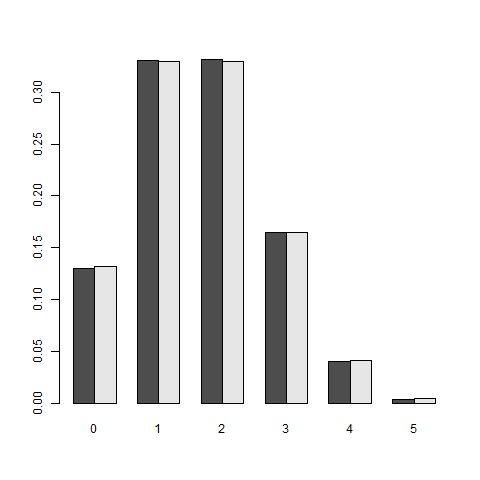
\includegraphics[width=8cm]{Barplot.png}
  \caption{Barplot of Distributions}
\end{figure*}
\newpage
\textit{Submit the code and the plot. Explain why you expect the probabilities to be close.}\\
\textbf{Answer:}\\
\begin{align*}
  p_H(x) &= \frac{{100 \choose x}{200 \choose {5-x}}}{{300 \choose 5}}\\
  &= {5 \choose x} \prod_{i=0}^{x-1}\frac{100-i}{300-i}\prod_{i=0}^{4-x}\frac{200-i}{300-x-i} 
\end{align*}
Let,
\begin{align*}
  p &= \frac{1}{3}\\
  p_1 &= \frac{100-x}{300-x}\\
  p_2 &= \frac{200-x}{300-5}
\end{align*}
Now,
$${5 \choose x}{p_1}^x(1-p_2)^{5-x} \leq p_H(x) \leq {5 \choose x}{p}^x(1-p_1)^{5-x}$$

As $300 \gg x$, $p_1 \approx p_2 \approx p = \frac{1}{3}$
$$\therefore p_H(x) \approx {5 \choose x}\biggl(\frac{1}{3}\biggr)^x\biggl(\frac{2}{3}\biggr)^{5-x} = p_B(x)$$
\vspace{4em}
\lstinputlisting[language=R, style=R, title=R Code for Histograms]{code.R}
\end{document}